\documentclass[a4paper]{article}
\title{MAT257---Analysis}
\author{Jonah Chen}

\usepackage[utf8]{inputenc}
\usepackage[margin=0.5in]{geometry}

\usepackage{braket}
\usepackage{physoly}
\usepackage{currfile}
\usepackage{gensymb}
\usepackage{amssymb}
\usepackage{pgf,tikz,pgfplots}
\usepackage{mathrsfs}
\usepackage{textcomp}
\usetikzlibrary{arrows}
\numberwithin{equation}{section}
\pgfplotsset{compat=1.16}

\newcommand{\R}{\mathbb{R}}

\begin{document}

\maketitle
\tableofcontents
\section{Course Overview}
\begin{itemize}
    \item $\mathbb R\to\mathbb R^n$
    \item Linear Algebra
    \item Continuity
    \item Differentiability
    \item Integration
    \item Key theorem of this class is \textbf{Stokes' Theorem}
    \begin{equation}
        \int_C\dd\omega=\int_{\partial C}\omega
    \end{equation}
    Generalizes the fundamental theorem of calculus:
    \begin{equation}
        \int_{[a,b]}F'(t)\dd t=F(b)-F(a)=\int_{\partial[a,b]}F
    \end{equation}
    Note that $\partial[a,b]=\{b+, a-\}$.
\end{itemize}

\section{Continuity}
\begin{itemize}
    \item Roughly speaking, continuity from $\mathbb R\to\mathbb R$ means if two points are near, their images should be near also.
    \item Thus, in $\mathbb R^n$, the intuitive meaning should be similar.
\end{itemize}
\subsection{Norms and Inner Product}
Note there are 2 conventions for $\mathbb R^n$
\begin{enumerate}
    \item The set of all n-dimensional real column vectors.
    \item The set of all n-dimensional real row vectors.
\end{enumerate}
In this class, the distinction is not very important.

\begin{definition}
    For $x, y\in\mathbb R^n$, "The standard (or euclidian) inner product of $x$ and $y$, denoted 
    \begin{equation}
        \langle x, y\rangle = \sum_{i=1}^n x_iy_i
    \end{equation}
    The norm-squared of $x$ is 
    \begin{equation}
        |x|^2=\langle x, x\rangle = \sum x_i^2
    \end{equation}
    and the norm of $x$ is
    \begin{equation}
        |x|=\sqrt{|x|^2} = \sqrt{\sum x_i^2}
    \end{equation}
\end{definition}

\begin{proposition}
    If $x, y, z\in\mathbb R^n$ and $a, b\in\mathbb R$, then
    \begin{enumerate}
        \item The inner product is bilinear \& the norm is ``semi-linear''.
        \begin{align}
                \langle ax+by,z \rangle &= a\langle x, z\rangle + b\langle y, z\rangle\\
            \langle z, ax+by \rangle &= \dots\\
            |ax|&=|a||x|
        \end{align}
        \textbf{Aside}: 
        \begin{equation}
            1=\sqrt 1=\sqrt{-1\cdot-1}=\sqrt{-1}\sqrt{-1}=i\cdot i=-1
        \end{equation}
        \item \begin{equation}
            |x|\geq 0 \& |x|=0\iff x=0
        \end{equation}
        \item \begin{equation}
            \langle x,y\rangle = \langle y,x \rangle
        \end{equation}
        \item \textit{Cauchy-Schwarz inequality}
        \begin{equation}
            |\langle x,y\rangle|\leq|x||y|
        \end{equation}
        with equality if $x\&y$ are dependent. 
        \item \textit{Triangle inequality}
        \begin{equation}
            |x+y|\leq |x|+|y|
        \end{equation}
        \item \textit{Polarization identity}
        \begin{equation}
            \langle x,y\rangle = \frac{|x+y|^2-|x-y|^2}{4}
        \end{equation}
    \end{enumerate}

    \begin{prooof}
        \begin{enumerate}
            \item $|x|=\sqrt{\sum x_i^2}$
            $|x|=0\implies\sum x_i^2=0\implies\forall i, x_i^2=0\implies \forall i,x_i=0\implies x=0$
            \item 
            For $s,t\in\mathbb R^n$
            \begin{equation}
                |s+t|^2=|s|^2+|t|^2+2\langle s,t \rangle
            \end{equation}
    
            Look at 
            \begin{align}
                0\leq\Big||y|^2x-\langle x,y\rangle y\Big|^2&=|y|^4|x|+\langle x,y\rangle^2|y|^2-2|y|^2\langle x,y\rangle^2\\
                &=|y|^2\left(|y|^2|x|^2-\langle x,y \rangle^2\right)
            \end{align}
            This is equal to zero only if $|y|^2x-\langle x,y\rangle y=0$. If we have equality, that implies $x\&y$ are dependent.
            \\\textbf{Why, what does this mean?}
            \item 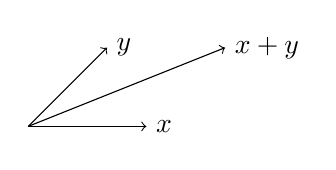
\begin{tikzpicture}
                \draw[->] (0,0) -- (1,1)node[anchor=west]{$y$};
                \draw[->] (0,0) -- (1.5, 0) node[anchor=west]{$x$};
                \draw[->] (0,0) -- (2.5, 1)node[anchor=west]{$x+y$};
            \end{tikzpicture}
            As both sides of the triangle inequality are $\geq0$, square both sides.
            \begin{align}
                |x+y|^2&\stackrel{?}{\leq}(|x|+|y|)^2\\
                \langle x+y, x+y \rangle&\stackrel{?}{\leq}|x|^2+|y|^2+2|x||y|\\
                \langle x,x\rangle + 2\langle x,y\rangle + \langle y,y\rangle &\stackrel{?}{\leq}|x|^2+|y|^2+2|x||y|\\
                |x|^2+|y|^2+2\langle x,y\rangle &\stackrel{?}{\leq}|x|^2+|y|^2+2|x||y|\\
                \langle x,y\rangle &\stackrel{?}{\leq}|x||y|\label{220}
            \end{align}
            \eqref{220} is true by cauchy-schwarz.
            \item The proof is trivial because you can expand the right hand side.
            \\\textbf{Note:} The inner product and the norm are not independent. If you know how to compute one, you can compute the other.
        \end{enumerate}
    \end{prooof}
\end{proposition}

\begin{definition}
    If $x, y\in\R^n$,define the distance between $x\&y$
    \begin{equation}
        d(x,y)=|x-y|
    \end{equation}
\end{definition}
\begin{theorem}
    \begin{enumerate}
        \item $d$ is symmetric: $d(x,y)=d(y,x)$
        \item $d$ is positive definite: $d(x,y)\geq0$ and $d(x,y)=0\iff x=y$
        \item Triangle inequality: $d(x,z)\leq d(x,y)+d(y,z)$
    \end{enumerate}
    The significance of this theorem is that this is all we need to know about distances to comment on continuity.\\
    \textbf{Aside:} Later, this theorem will become a definition for a distance function or a metric.
    \begin{prooof}
        \begin{enumerate}
            \item \begin{align}
                d(x,y)=|x-y|=|-(y-x)|=|-1||y-x|=|y-x|=d(y,x)
            \end{align}
            \item \begin{align}
                d(x,y)=0\iff |x-y|=0\iff x-y=0\iff x=y
            \end{align}
            \item \begin{align}
                |x-z|\stackrel{?}{\leq}|x-y|+|y-z|
            \end{align}
            This is true by the previous triangle inequality, $|p|+|q|\geq|p+q|$. Letting $p=x-y,q=y-z\implies p+q=x-z$.
        \end{enumerate}
    \end{prooof}

    There are other norms and distance functions that we will rarely use.

    \begin{itemize}
        \item The euclidian norm which we use is $|x|_{L^2}=\sqrt{\sum x_i^2}$.
        \item There is a L1 norm $|x|_{L^1}=\sum|x_i|$.
        \item The L-infinity norm is $|x|_{L^\infty}=\max |x_i|$.
    \end{itemize}
    The distance functions for these norms also satisfys these three properties.
\end{theorem}




\end{document}
